% Options for packages loaded elsewhere
\PassOptionsToPackage{unicode}{hyperref}
\PassOptionsToPackage{hyphens}{url}
\PassOptionsToPackage{dvipsnames,svgnames,x11names}{xcolor}
\documentclass[
  10pt,
  fontset=fandol]{ctexart}
\usepackage{xcolor}
\usepackage[margin=16mm]{geometry}
\usepackage{amsmath,amssymb}
\setcounter{secnumdepth}{-\maxdimen} % remove section numbering
\usepackage{iftex}
\ifPDFTeX
  \usepackage[T1]{fontenc}
  \usepackage[utf8]{inputenc}
  \usepackage{textcomp} % provide euro and other symbols
\else % if luatex or xetex
  \usepackage{unicode-math} % this also loads fontspec
  \defaultfontfeatures{Scale=MatchLowercase}
  \defaultfontfeatures[\rmfamily]{Ligatures=TeX,Scale=1}
\fi
\usepackage{lmodern}
\ifPDFTeX\else
  % xetex/luatex font selection
\fi
% Use upquote if available, for straight quotes in verbatim environments
\IfFileExists{upquote.sty}{\usepackage{upquote}}{}
\IfFileExists{microtype.sty}{% use microtype if available
  \usepackage[]{microtype}
  \UseMicrotypeSet[protrusion]{basicmath} % disable protrusion for tt fonts
}{}
\makeatletter
\@ifundefined{KOMAClassName}{% if non-KOMA class
  \IfFileExists{parskip.sty}{%
    \usepackage{parskip}
  }{% else
    \setlength{\parindent}{0pt}
    \setlength{\parskip}{6pt plus 2pt minus 1pt}}
}{% if KOMA class
  \KOMAoptions{parskip=half}}
\makeatother
\usepackage{longtable,booktabs,array}
\newcounter{none} % for unnumbered tables
\usepackage{calc} % for calculating minipage widths
% Correct order of tables after \paragraph or \subparagraph
\usepackage{etoolbox}
\makeatletter
\patchcmd\longtable{\par}{\if@noskipsec\mbox{}\fi\par}{}{}
\makeatother
% Allow footnotes in longtable head/foot
\IfFileExists{footnotehyper.sty}{\usepackage{footnotehyper}}{\usepackage{footnote}}
\makesavenoteenv{longtable}
\usepackage{graphicx}
\makeatletter
\newsavebox\pandoc@box
\newcommand*\pandocbounded[1]{% scales image to fit in text height/width
  \sbox\pandoc@box{#1}%
  \Gscale@div\@tempa{\textheight}{\dimexpr\ht\pandoc@box+\dp\pandoc@box\relax}%
  \Gscale@div\@tempb{\linewidth}{\wd\pandoc@box}%
  \ifdim\@tempb\p@<\@tempa\p@\let\@tempa\@tempb\fi% select the smaller of both
  \ifdim\@tempa\p@<\p@\scalebox{\@tempa}{\usebox\pandoc@box}%
  \else\usebox{\pandoc@box}%
  \fi%
}
% Set default figure placement to htbp
\def\fps@figure{htbp}
\makeatother
\setlength{\emergencystretch}{3em} % prevent overfull lines
\providecommand{\tightlist}{%
  \setlength{\itemsep}{0pt}\setlength{\parskip}{0pt}}
\usepackage{amsmath,amssymb,mathtools,needspace}
\xeCJKDeclareCharClass{CJK}{"2032,"0400->"04FF,"2160->"216B,"2460->"2473,"25A0,"25C7,"25CB,"25CF}
\IfFontExistsTF{Arial Unicode MS}{\xeCJKsetup{AutoFallBack=true}\setCJKfallbackfamilyfont{\CJKrmdefault}{Arial Unicode MS}}{}
\setcounter{secnumdepth}{0}
\setlength{\emergencystretch}{2em}
\allowdisplaybreaks
\usepackage{bookmark}
\IfFileExists{xurl.sty}{\usepackage{xurl}}{} % add URL line breaks if available
\urlstyle{same}
\hypersetup{
  pdftitle={Chebyshev 多项式},
  colorlinks=true,
  linkcolor={Maroon},
  filecolor={Maroon},
  citecolor={Blue},
  urlcolor={Blue},
  pdfcreator={LaTeX via pandoc}}

\title{Chebyshev 多项式}
\author{}
\date{}

\begin{document}
\maketitle

\subsubsection{3.4.3 Chebyshev多项式}\label{chebyshevux591aux9879ux5f0f}

当权函数 \(\rho(x) = \frac{1}{\sqrt{1-x^2}}\), 区间为 \([-1, 1]\) 时, 由序列 \(\{1,\allowbreak  x,\allowbreak  x^2,\allowbreak  \cdots,\allowbreak  x^n,\allowbreak  \cdots\}\) 正交化得到的正交多项式就是 Chebyshev多项式, 它可表示为 \[
T_n(x) = \cos(n \arccos x), \quad |x| \leqslant 1. \tag{3.4.6}
\] 若令 \(x = \cos \theta\), 则 \[
T_n(x) = \cos n \theta, \quad 0 \leqslant \theta \leqslant \pi.
\] Chebyshev多项式有很多重要性质.

性质 1 递推关系 \[
T_0(x) = 1, \quad T_1(x) = x,
\] \[
T_{n+1}(x) = 2xT_n(x) - T_{n-1}(x) \quad (n = 1, 2, \cdots). \tag{3.4.7}
\] 这只要由三角恒等式 \[
\cos(n+1)\theta = 2\cos \theta \cos n \theta - \cos(n-1)\theta \quad (n \geqslant 1)
\] 令 \(x = \cos \theta\) 即得. 由式(3.4.7)可得表 3.1.

\(T_n(x)\) 的函数图形如图 3.5 所示.

表 3.1

{\def\LTcaptype{none} % do not increment counter
\begin{longtable}[]{@{}ll@{}}
\toprule\noalign{}
多项式 & 表达式 \\
\midrule\noalign{}
\endhead
\bottomrule\noalign{}
\endlastfoot
\(T_0(x)\) & \(1\) \\
\(T_1(x)\) & \(x\) \\
\(T_2(x)\) & \(2x^2-1\) \\
\(T_3(x)\) & \(4x^3-3x\) \\
\(T_4(x)\) & \(8x^4-8x^2+1\) \\
\(T_5(x)\) & \(16x^5-20x^3+5x\) \\
\(T_6(x)\) & \(32x^6-48x^4+18x^2-1\) \\
\(T_7(x)\) & \(64x^7-112x^5+56x^3-7x\) \\
\(T_8(x)\) & \(128x^8-256x^6+160x^4-32x^2+1\) \\
\end{longtable}
}

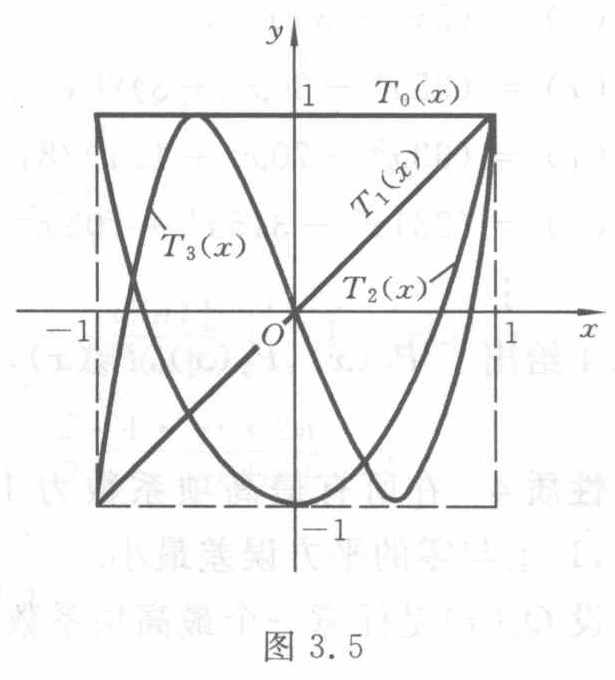
\includegraphics[width=0.85\linewidth,height=\textheight,keepaspectratio,alt={图 3.5 原图裁切}]{../assets/ch03a/fig-3-5.png}

图 3.5（原图）。Chebyshev 多项式 \(T_0(x)\)、\(T_1(x)\)、\(T_2(x)\)、\(T_3(x)\) 的图形。全部标签：\(x\)、\(y\)、\(O\)、横轴的 \(-1\)、\(1\)、纵轴的 \(1\)、\(-1\)、\(T_0(x)\)、\(T_1(x)\)、\(T_2(x)\)、\(T_3(x)\)；在 \(x=\pm1\) 处画有辅助线。

\href{../../source-images/pdf-074.jpeg}{查看原页}

由递推关系式(3.4.7)还可得到 \(T_n(x)\) 的最高项系数是 \(2^{n-1}(n \geqslant 1)\).

性质 2 \(T_n(x)\) 对零的偏差最小. 它可写成如下定理.

定理 3.7 在区间 \([-1,1]\) 上所有最高项系数为 1 的一切 \(n\) 次多项式中, \(\omega_n(x) = \frac{1}{2^{n-1}} T_n(x)\) 与零的偏差最小, 其偏差为 \(\frac{1}{2^{n-1}}\).

证明 由于 \(\omega_n(x) = \frac{1}{2^{n-1}} T_n(x) = x^n - P_{n-1}^*(x)\),

\[
\max_{-1 \leqslant x \leqslant 1} |\omega_n(x)| = \frac{1}{2^{n-1}} \max_{-1 \leqslant x \leqslant 1} |T_n(x)| = \frac{1}{2^{n-1}} ,
\] 且点 \(x_k = \cos \frac{k}{n}\pi (k=0,1,\cdots,n)\) 是 \(T_n(x)\) 的 Chebyshev 交错点组, 由定理 3.4 可知, 在区间 \([-1,1]\) 上, \(x^n\) 在 \(H_{n-1}\) 中最佳逼近多项式为 \(P_{n-1}^*(x)\), 即 \(\omega_n(x)\) 是与零的偏差最小的多项式. 证毕.

例 3.3 求 \(f(x) = 2x^3 + x^2 + 2x - 1\) 在 \([-1,1]\) 上的最佳二次逼近多项式.

解 由题意, 所求最佳逼近多项式 \(P_{2}^*(x)\) 应满足

\[
\max_{-1 \leqslant x \leqslant 1} |f(x) - P_{2}^*(x)| = \min .
\] 由定理 3.6 可知, 当

\[
f(x) - P_{2}^*(x) = \frac{1}{2} T_3(x) = 2x^3 - \frac{3}{2}x
\] 时, 与零偏差最小, 故

\[
P_{2}^*(x) = f(x) - \frac{1}{2} T_3(x) = x^2 + \frac{7}{2}x - 1
\] 就是 \(f(x)\) 在 \([-1,1]\) 上的最佳二次逼近多项式.

性质 3 Chebyshev 多项式 \(\{T_k(x)\}\) 在区间 \([-1,1]\) 上带权 \(\rho(x) = 1 / \sqrt{1-x^2}\) 正交, 且

\[
\int_{-1}^{1} \frac{T_n(x)T_m(x)\,\mathrm{d}x}{\sqrt{1-x^2}} = \begin{cases} 0, & n \neq m, \\ \frac{\pi}{2}, & n = m \neq 0, \\ \pi, & n = m = 0. \end{cases} \tag{3.4.8}
\]

事实上, 令 \(x = \cos \theta\), 则 \(\mathrm{d}x = -\sin \theta \mathrm{d}\theta\), 于是

\[
\int_{-1}^{1} \frac{T_n(x)T_m(x)}{\sqrt{1-x^2}} \mathrm{d}x = \int_{0}^{\pi} \cos n\theta \cos m\theta \mathrm{d}\theta = \begin{cases} 0, & n \neq m, \\ \frac{\pi}{2}, & n = m \neq 0, \\ \pi, & n = m = 0. \end{cases}
\]

性质 4 \(T_{2k}(x)\) 只含 \(x\) 的偶次幂, \(T_{2k+1}(x)\) 只含 \(x\) 的奇次幂.

此性质由递推关系直接得到.

\begin{quote}
校注（agent 补充，原书交叉引用疑误）：例 3.3 中原文写``由定理 3.6 可知''，照录。此处使用的是本页定理 3.7 的最小偏差性质；定理 3.6 是线性无关与内积行列式的判别条件。
\end{quote}

\href{../../source-images/pdf-075.jpeg}{查看原页}

性质 5 \(T_n(x)\) 在区间 \([-1,1]\) 上有 \(n\) 个零点 \(x_k = \cos \frac{2k-1}{2n}\pi, k=1, \cdots, n\). 此外, 实际计算中时常要求 \(x^n\) 用 \(T_0, T_1, \cdots, T_n\) 的线性组合表示, 其公式为 \[
x^n = 2^{1-n} \sum_{k=0}^{[\frac{n}{2}]} \binom{n}{k} T_{n-2k}(x). \tag{3.4.9}
\]

这里规定 \(T_0 = 1/2\). \(n=1 \sim 8\) 的结果如表 3.2 所示.

表 3.2

{\def\LTcaptype{none} % do not increment counter
\begin{longtable}[]{@{}ll@{}}
\toprule\noalign{}
幂函数 & Chebyshev 多项式表示 \\
\midrule\noalign{}
\endhead
\bottomrule\noalign{}
\endlastfoot
\(1\) & \(T_0\) \\
\(x\) & \(T_1\) \\
\(x^2\) & \(\frac12(T_0+T_2)\) \\
\(x^3\) & \(\frac14(3T_1+T_3)\) \\
\(x^4\) & \(\frac18(3T_0+4T_2+T_4)\) \\
\(x^5\) & \(\frac1{16}(10T_1+5T_3+T_5)\) \\
\(x^6\) & \(\frac1{32}(10T_0+15T_2+6T_4+T_6)\) \\
\(x^7\) & \(\frac1{64}(35T_1+21T_3+7T_5+T_7)\) \\
\(x^8\) & \(\frac1{128}(35T_0+56T_2+28T_4+8T_6+T_8)\) \\
\end{longtable}
}

\begin{center}\rule{0.5\linewidth}{0.5pt}\end{center}

\subsection{相关原页校注（agent 补充）}\label{ux76f8ux5173ux539fux9875ux6821ux6ce8agent-ux8865ux5145}

以下校注来自本节覆盖的原页，可能也涉及同页相邻小节；原文照录与校正说明分开保留。

\subsubsection{原书 PDF 页 75 的校注}\label{ux539fux4e66-pdf-ux9875-75-ux7684ux6821ux6ce8}

\href{../pages/pdf-075.md}{完整原页转录} · \href{../../source-images/pdf-075.jpeg}{原页图像}

\begin{quote}
校注（agent 补充，记号约定）：式 (3.4.9) 后原文规定 \(T_0=1/2\)，而表 3.2 首行原印 \(1=T_0\)；两处均忠实保留。式 (3.4.9) 的求和使用临时的半权常数项约定，表 3.2 则与前文通常定义 \(T_0=1\) 一致。使用时须区分这两种约定。
\end{quote}

\subsection{本节覆盖原页的校注记录}\label{ux672cux8282ux8986ux76d6ux539fux9875ux7684ux6821ux6ce8ux8bb0ux5f55}

下列记录按原页关联，含同页相邻小节的校注；计算时同时读取上文校注和完整原页。

\begin{itemize}
\tightlist
\item
  \texttt{ch03a-E11}：原书 PDF 页 74
\end{itemize}

\end{document}
